\documentclass{jsarticle}

\usepackage{graphicx}
\usepackage{latexsym}
\usepackage{amsmath}
\usepackage{amssymb}
\usepackage{amsthm}
\usepackage{url}
\usepackage{algorithm}
\usepackage{algorithmicx}
\usepackage{algpseudocode}
\newcommand{\argmin}{\operatornamewithlimits{argmin}}
\newcommand{\dd}{\mathrm{d}}
\newcommand{\ee}{\mathrm{e}}

\theoremstyle{definition}
\newtheorem{thm}{定理}
\newtheorem{defi}[thm]{定義}
\newtheorem{prop}[thm]{命題}
\newtheorem{cor}[thm]{系}
\newtheorem{asm}[thm]{仮定}

\renewcommand{\algorithmicrequire}{\textbf{Input:}}
\renewcommand{\algorithmicensure}{\textbf{Output:}}

\title{質問者のプライバシーを保護する特許データベース検索 \\(文献紹介)}
\author{中川研究室 修士2年 胡 瀚林\\指導教員: 中川 裕志 教授}
\date{2016年7月1日}

\begin{document}
\maketitle
\begin{abstract}
企業が特許を取る前に,類似な特許が既に存在するかを確かめるために特許データベースを検索する必要がある.
しかし,検索の質問から企業秘密が漏洩する可能性がある.
また一般的なウェブテキスト検索と違い,特許データベース検索は長い検索質問を用い,検索の精度と再現率を重視している.
紹介文献\cite{pang_embellishing_2010}では直接質問者の質問にデミー単語を混ぜて質問のある種の匿名性を保証し,準同型暗号を用いて文章と真の質問単語の関連性スコアけを計算できる検索スキームより検索の精度と再現率を維持する.

本発表では\cite{pang_embellishing_2010}を紹介して,潜在的意味インデキシングを用いる攻撃手法を提案し,特許データベースを用いて提案手法を評価する.
\end{abstract}

\section{はじめに}
テキスト検索をするとき,検索質問をサーバー側に渡さなければならない.しかし,検索質問からユーザーの情報が漏洩する危険があることがAOL事件\cite{_face_2006}より証明された.特に特許検索の場合は質問が研究開発動向など企業秘密を含んでいるため,一般的なウェブ検索のユーザーよりテキスト検索のプライバシー問題を重視している.

今テキスト検索エンジンの大半が類似検索である.全ての質問単語を含んでいる文章しか検索できないキーワード検索と違い,類似検索は文章と質問の関連性を計算し文章にランクをつける\cite{zobel_inverted_2006}.毎回全ての文章との関連性を計算しないために検索エンジンが単語と文章の関連値を転置ファイルに保存し,質問の単語と文章の関連値の和を質問とその文章の関連性とする.このような計算が必要であるため,\cite{bethencourt_new_2006},\cite{freedman_keyword_2005},\cite{boneh_public_2004},\cite{song_practical_2000}などキーワード検索だけ対応できる研究は類似検索に応用できない.また質問のある種の匿名性より質問者のプライバシーを保護する手法がある.\cite{murugesan_providing_2009}では事前的に静的な質問セットを作り,真の質問$q$の代わりに真の質問と一番類似な質問$q'$を含んでいる質問セットをサーバーに送る.$q'$が真の質問の大半な結果を検索できると考えられ,質問セット中の他の質問をダミー質問にする.そのため,このメカニズムは検索の精度と再現率に影響を大きく与える.また,質問の長さの増加と伴って質問の可能な組み合わせが指数的に増加するため,実践的には特許検索など長い質問が多いテキスト検索と質問拡張\cite{qiu_concept_1993,xu_query_1996}に対応できない.

\cite{pang_embellishing_2010}では長い質問と類似検索に対応できるメカニズムを提案した.本稿の構成は次の通りである.第二章では背景知識を述べる.第三章では\cite{pang_embellishing_2010}に提案したメカニズムを述べる.第四章ではそのメカニズムに対する攻撃手法を提案し,特許データベースを用いて\cite{pang_embellishing_2010}の安全性を検証する.最後に, 第六章で全体をまとめる.


\section{準備}
本章では類似検索,準同型暗号,潜在的意味インデキシング,攻撃モデルの順に関連知識と関連研究を述べる.

\subsection{類似検索}
コーパス$\mathcal{D}$における検索エンジンが質問を処理するとき基本的には転置ファイルを用いている.転置フィルは質問単語の辞書$\mathcal{T}$と全ての単語の転置リストからなる.単語$t_i \in \mathcal{T}$の転置リスト$L_i$が$\langle d_i,p_{ij}\rangle$の列である.$p_{ij \in \Re}$は単語$t_i$と文章$d_i \in \mathcal{D}$の関連性である.$t_i$が$d_i$に現れたなら$p_{ij}$の値は$0$より大きい,現れなかったなら$0$となる.空間圧縮のために$p_{ij}=0$な$d_i$は$L_i$に含まれていない.

質問$q=\{t_i\}$と文章$d_i$と関連性は以下のように計算する
\begin{equation}
S_{d_j,q} = \sum_{t_i \in q}p_{ij}
\end{equation}
したがって転置リスト$L_i$に含まれている文章だけが$0$以上のスコアを持ち,$q$と関連があると見なす.転置フィルを全体暗号化しても,サーバーは転置リストの長さとアクセス頻度などの情報から真の関係値を推定できるため,そのような方法は無意味だと考えられる.

\subsection{準同型暗号}\label{enc}
二つの暗号文 $E(m_1), E(m_2)$ が与えられた時に、平文や秘密鍵なしで $E( m_1 \circ m_2 )$を計算できる暗号を準同型暗号と呼ぶ.紹介文献ではBenalohの加算可能な準同型暗号\cite{benaloh_dense_1994}を用いた.Benaloh暗号は以下のように$[1,r-1]$中のメッセージを暗号化する.\\
鍵生成,\\
1.$(p_1-1)$が$r$に整除でき,$(p_1-1)/r$と$r$が互いに素であり,$(p_2-1)$と$r$が互いに素であるように大きい素数$p_1$と$p_2$を選ぶ.\\
2.$n = p_1p_2$\\
3.$g^{(p_1-1){p_2-1}/r} \, mod \, n \neq 1$のようになる$g \in \mathbb{Z}^*_n$を選ぶ.\\
4.$(n,q)$が公開鍵であり,$(p_1,p_2)$が秘密鍵である.\\
暗号化,\\
1.$\mu \in \mathbb{Z}^*_n$をランダムに選ぶ.
2.$E(m) = g^m\mu^r \, mod \, n$.\\
乱数$\mu$により同じメッセージ$m$が複数の暗号文に対応でき,攻撃者が暗号文の頻度から$m$を推定することを防げる.

暗号文$E(m)$を復号するため,全ての$i \in \mathbb{Z}_r$を以下の式を満たすかどうかを確かめる必要がある,
\begin{equation}
(g^{-i} \cdot E(m))^{(p_1-1){p_2-1}/r} = 1 \, mod \, n
\end{equation}
$m=i$のときだけ上記を式が満たす.$g^{-i} mod \, n $が事前的に計算できる.

$E(m_1)\cdot E(m_2) = g^{m_1m_2}{\mu_1\mu_2}^r \, mod \, n = E(m_1 + m_2)$.したがってBenaloh暗号は加算可能な準同型暗号である.

\subsection{潜在的意味インデキシング}\label{LSI}
特異値分解 (SVD) を用いて単語をトピック空間にマップすることが潜在的意味インデキシング(LSI)\cite{deerwester_indexing_1990}の基礎である.
LSIではトピック空間中の単語と文書の関係を用いて多義性と同義性の問題を解決する.
つまり、 綴りが違うが同じような意味を持つ単語はトピック空間での距離が近いようにできる.

単語$\cdot$文書行列$A$の$(i,j)$番目の要素は$i$番目の単語が$j$番目の文章に出現した回数である.
$A$を特異値分解$A = USV^T$し、$U$、$S$、$V$	の各列ベクトルを特異値が大きい順に$K$個用いて$A$の低ランク近似$A_K=U_KS_KV_{K}^T$を得る.
このように低ランク分解によって、単語とトピックの関係を分析できる.
$A_K$の$(i,j)$番目の要素は$i$番目の単語と$j$番目のトピックの関係を表す.
その値が大きければ大きいほど単語とピックの関係が強い.
本発表では単語$i$と対応する行列$A_K$の行$\ell_i$を単語$i$のトピックベクトルと呼ぶ.

\subsection{攻撃モデル}
本発表では検索サーバーが攻撃者だと仮定する.
検索サーバーがデータベースの全ての情報を持つため,可能な攻撃者の中で一番強いと考えられる.
また攻撃者が二種類のモデルに分類できる.
Semi-honestな攻撃者はプロトコルには従うが,イデアルモデルで得られる以上の情報を得ようと試みる.
Maliciousな攻撃者は任意のやり方でプロトコルから逸脱したり,入力を偽ったり,任意時点で停止したりする.
本発表では,semi-honestなサーバーが攻撃者であることを前提としてプライバシー問題を分析する.

\begin{table}[!hbp]
\center
\begin{tabular}{|c|c|}
\hline
符号 & 意味 \\
\hline
$N$ & 辞書中の単語の数 \\
$t_i$ & 辞書中$i$番目の単語 \\
$L_i$ & 単語$t_i$の転置リスト \\
$d_j$ & コーパス中$j$番目の文章 \\
$score_j$ & $d_j$の関連性スコア \\
Bkts & 単語バケツの数 \\
BktSz & 単語バケツ中の単語の数 \\
SegSz & セグメント中の単語の数 \\
$\ell_i$ & 単語$t_i$のトピックベクトル \\
$\ell$ & 質問のトピックベクトル \\
$E(\cdot)$ & Benaloh加算可能準同型暗号化 \\
\hline
\end{tabular}
\caption{表記法}
\end{table}

\section{テキスト検索質問を加工して質問者のプライバシーを保護する}
テキスト検索質問は単語の集合である.
\cite{murugesan_providing_2009}など質問にダミーを混ぜて同時に検索する曖昧化検索(Obfuscation Search)の既存研究は質問の全体を分析し,適切な$K-1$個のダミー質問を選ぶ.
質問の全体ではなく単語ごとにダミー単語を混ぜれば,真の質問である可能性がある質問数が増え,攻撃者が真の質問を見破る確率が下がる.
質問者がいつのトピックに対して検索するとき,一つの単語を複数回使うと考えられる.
毎回違うダミー単語を混ぜると同じ質問者の質問に出る頻度が高い単語が真の質問単語となる可能性が頻度が低い単語より大きくなる.
そんなリスクを防ぐため紹介文献では単語バケツを事前的に作り,真の質問単語と同じバケツにある他の単語をダミー単語とする.

\subsection{単語バケツ}
単語バケツを作るには2つ主要なリスクがある.
真の質問単語が全て同じトピックについて述べると考えられる.そのような単語がランダムに選んだダミー単語と区別することが簡単である.
また特許検索に多く使っている専攻用語など特殊な単語と一般的よく使っている単語を混ぜると,専攻用語が真の質問である可能性が大きいと考えられる.
そんなリスクを減らすために,以下の特徴を持つ単語バケツを作りたい:
(1)同じバケツにある単語の特殊さは近いが,意味的には大きい違いがある.
(2)2つのバケツの全ての単語間の意味的距離の差が近い.
\label{risk}
検索するとき,質問単語が属するバケツ中他の単語がダミー単語として質問に加える.
したがって特殊な単語のダミー単語がいつも同じような特殊さを持ち,デミー単語間の関係が真の質問の単語間の関係が似ていると考えられる.

紹介文献では単語を類義関係のセット(synset)でグループ化し、一つのsynsetが一つの概念に対応し,各synsetは上位下位関係,全体部分関係などの関係でリンクされているWordNet\cite{miller_wordnet:_1995}を用いて単語バケツを作る.

2つ単語が属するsynset間の最短パスを単語間の意味的距離とする.
また上位下位関係でリンクされた2つsynsetの中下位語が上位語より特殊であると考えられる.
WordNetの中で実体(entity)以外全部の名詞synsetの上位語が唯一に存在する.
上下位関係を枝とすると、WordNet中の名詞synsetが実体を根とする木となる.
単語が属する一番深さが浅いsynsetの深さを単語の特殊レベルとし,レベルが大きければ大きいほど単語が特殊である.

\subsection{バケツ作り}
\begin{algorithm}
\caption{単語を一列に並べる}
\begin{algorithmic}[1]
\Function{ProcessSynset}{synset ss}
	\If {$ss$の単語が複数の既存な単語列に含まれている}
	\State そんな単語列を結合する
	\State 結合した単語列を$sq$にする
	\ElsIf {$ss$の単語が既存な単語列に含まれていない}
	\State 新たの単語列を作る
	\Else {\, $ss$の単語の一つが一つ既存な単語列に含まれている}
	\State その単語列を$sq$にする
	\EndIf
	\State 処理していない$ss$の単語を$sq$に加える
	\State $ss$の単語を処理したとマークする
	\State $ss$を処理したとマークする
	\State 単語列$sq$を返す 
\EndFunction
\Function{SequenceVocab}{WordNet wndb}
	\State 全てのsynsetを関係数が多い方から小さい方への順で並べる
	\State 全てのsynsetを処理していないとマークする
	\State 全ての単語を処理していないとマークする
	\State $SeqSet = \phi$
	\ForAll {処理していないsynset $ss$}
		\State $sq=ProcessSynset(ss)$;$sq$を$SeqSet$に加える
		\ForAll {$ss$と反意関係,上位下位関係,全体部分関係をもつsynset $ss'$}
		\State 処理していない$ss'$の単語を$sq$に加える
		\State $ss'$の単語を処理したとマークする
		\State $sq=ProcessSynset(ss')$;$sq$を$SeqSet$に加える 
		\EndFor
	\EndFor
\EndFunction
\end{algorithmic}
\end{algorithm}

本節では単語バケツを作る方法を述べる.
まずアルゴリズム1を用いてWordNetデータベース中の意味的近い単語を隣にして全ての単語一列に並べる.
リンクが多いsynsetが意味的に豊富であるため,単語を一列に繋がる種として使われ,synsetの関係数が多い方から小さい方への順で処理する.
複数の意味を持つ単語が属するsynsetが意味的近いと考え,同じ単語を持つsynsetを隣に並べる.
また反意関係,上位下位関係,全体部分関係を持つsynsetを隣に並べる.
2つの操作により,列に近い単語の意味も近いと保証する.

WordNetデータベースにアルゴリズム1を行った結果データベース中全ての$117,798$個の名詞を一列に並べ,アルゴリズムに有効性を証明した.

\begin{figure}[!hbp]
    \centering
    \includegraphics[width=0.8\textwidth,natwidth=5677,natheight=1982]{rk11.png}
	\caption{バケツ作り-$N=1000,BktSz=2$}\label{fig:pp1}
\end{figure}

\begin{algorithm}
\caption{単語列から単語バケツを作る}
\begin{algorithmic}[1]
\Function{GenerateBuckets}{sq,BktSz,Segsz}
	\State $N=$単語列$sq$の長さ
	\State $\#Seg=N/SegSz$
	\State $sq$を同じ長さのセグメントに分割する$S_1,S_2, \dots , S_{\#Seg}$
	\State セグメント中の単語を特殊レベルが大きい方から小さい方への順で再配列する
	\For {$i = 1 to N/(BktSz * SegSz)$}
	\State ActiveSeg = $\phi$
		\For {$j = 1 to BktSz$}
		\State $ActiveSeg = ActiveSeg \cup S_{(j-1)N/(BktSz * SegSz)}$
		\EndFor
		\For {$j = 1 to SegSz$}
		\State 新たなバケツ$B=\phi$を作る
		\State ActiveSeg中の全てのセグメントの$j$番目の単語を$B$に入れる
		\State $B$を出力する
		\EndFor
	\EndFor
\EndFunction
\end{algorithmic}
\end{algorithm}

次ではアルゴリズム1で出力した単語列を単語バケツにする.
アルゴリズム2がその過程を表している.
バケツの大きさを$1 \leq$BktSz$\leq N$に設定する.
バケツの数が\#Bkts$=N/$BktSzである.
同じバケツ中の単語を可能な限りに違う意味にするために単語列の$1,\#$BktSz$+1,2*\#$BktSz$+1, \dots,($BktSz$-1)*\#$BktSz$+1$番目の単語をバケツ1に,$2,\#$BktSz$+2,2*\#$BktSz$+2, \dots,($BktSz$-1)*\#$BktSz$+2$をバケツ2に,$i,\#$BktSz$+i,2*\#$BktSz$+i, \dots,($BktSz$-1)*\#$BktSz$+i$をバケツ$i$に入れる.
図\ref{fig:pp1}が$N=1000,BktSz=2$のときのバケツ作り過程を表している.
その操作により,2つのバケツ$i$と$j$の同じ位置の単語間の距離が同じ$\|i-j\|$であり,意味的な距離の差も小さいと考えられる.
またバケツ同じ位置の単語間の距離が違う位置の単語間の距離より近いため、真の質門の単語が同じ位置にあると仮定する。
したがって,真の質問の単語が意味的に近いときあるいは一つのトピックに集中したとき,バケツの中のダミー単語も同じように一つのトピックに集中すると考えられる.
しかし,バケツ中の単語の特殊レベルがランダムであり,大きく違う可能性がある.

バケツ中の単語の特殊レベルを調整するために,隣接のバケツ間の単語交換を行う.
実践的には単語を単語バケツに配置する前に単語列を同じ長さSegSz$\leq N/$BktSzのセグメントに分割し,セグメント内の単語を特殊レベルが大きい方から小さい方への順で再配列する.
SegSzがBktSzの整数倍である必要がある.
図\ref{fig:pp2}が図\ref{fig:pp1}の上に単語列の再配列を加えた流れを表している.
その結果,同じバケツにある単語のセグメント内の順番が同一であり,特殊レベルが近くなると考えられる.


バケツ作りには2つのパラメータを設定する必要ある.
SegSzが2つのリスクのトレードオフとなる.
SegSzが増加することは単語交換を行う範囲が増大することに相当する.
SegSzが大きければ大きいほどバケツ中の単語の特殊レベルが近くなる.
一方、単語間の意味的な距離も近くなる可能性がある.
もう一つのパラメータBktSzがプライバシーと計算時間のトレードオフとなる.
BktSzが大きくなると,真の質問を特定する可能性が下がるが,検索エンジンが処理する質問単語が増加する.
SegSzとBktSzを影響は\ref{ex}節で述べる.

\begin{figure}
    \centering
    \includegraphics[width=0.5\textwidth,height=0.3\textwidth,natwidth=1600,natheight=1196]{rk13.png}
	\caption{バケツ作り-$N=1000,BktSz=2,SegSz=4$}\label{fig:pp2}
\end{figure}

\subsection{プライベート検索スキーム}
本節では真の質問単語だけの関連性スコアを計算できる検索スキームを述べる.
検索スキームは質問加工,質問検索と結果処理三部分からなる.

\begin{algorithm}
\caption{質問加工}
\begin{algorithmic}[1]
\Function{GenerateBuckets}{sq,BktSz,Segsz}
	\Require 真の質問単語$t_i$の集合
	\Ensure 加工した質問$q$
	\ForAll {真の質問単語$t_i$}
	\State Bkt$=t_i$が属する単語バケツ
		\ForAll {$t_j \in $Bkt}
		\If {$t_i == t_j$} $\mu_j=1$
		\Else $\,\mu_j=0$
		\EndIf
		\State $E(u_j) = g^{\mu_j}\mu^r$
		\State $\langle t_j,E(\mu_j)\rangle$を$q$に入れる
		\EndFor
	\EndFor
\EndFunction
\end{algorithmic}
\end{algorithm}

アルゴリズム3が質問加工の流れを表す.
真の質問単語が属するバケツの中の他の単語を全てデミー単語として質問に加える.
デミーを加えた質問の単語$t_j$に$E(\mu_j)$を付け,$t_j$が真の質問単語なら$\mu_j=1$,ダミー単語なら$\mu_j=0$.
$E(\cdot)$が\ref{enc}節で紹介した暗号化関数である.
加工した質問$q$をサーバーに送る.

\begin{algorithm}
\caption{質問検索}
\begin{algorithmic}[1]
\Function{GenerateBuckets}{sq,BktSz,Segsz}
	\Require 加工した質問$q$
	\Ensure 文章とその文章暗号文した関連性スコアの集合$R$
	\State $R=\phi$
	\ForAll {$\langle t_i,E(\mu_i)\rangle \in q$}
		\ForAll {$\langle d_j,p_{ij}\rangle \in L_i$}
		\If {$\exists \langle d_j,E(score_j)\rangle \in R$} 
		\State $E(score_j)=E(score_j)*E(\mu_j)^{p_{ij}}$
		\Else 
		\State $\langle t_j,E(\mu_j)^{p_{ij}}\rangle$を$R$に入れる
		\EndIf
		\EndFor
	\EndFor
\EndFunction
\end{algorithmic}
\end{algorithm}

アルゴリズム4がサーバー側の検索過程を表す.
サーバーが単語と文章の関連値を保存している転置フィルを用いて文章の関連性スコアを計算する.
加算可能な準同型暗号の特徴より,$E(\mu_j)^{p_{ij}}=E(\mu_j*p_{ij})$.
$t_j$がダミー単語であれば,$E(score_j)*E(\mu_j)^{p_{ij}}=E(score_j)*E(0*p_{ij})=E(score_j)$.
復号した関連性スコアには影響を与えない.
したがって,$score_j$が真の質問単語と文章の関連値$p_{ij}$の和となる.

\begin{algorithm}
\caption{結果処理}
\begin{algorithmic}[1]
\Function{GenerateBuckets}{sq,BktSz,Segsz}
	\Require 文章とその文章暗号文した関連性スコアの集合$R$
	\Ensure 順番順序付けらた文章列
	\State $R=\phi$
	\ForAll {$ \langle d_j,E(score_j)\rangle \in R$}
		\State $E(score_j)$を$score_j$に復号する
	\EndFor
	\State $R$中の文章を関連性スコアが大きい方から小さい方への順で並べる
	\State $R$中上位の文章を返す
\EndFunction
\end{algorithmic}
\end{algorithm}

最後に質問者がサーバーがらもらった結果集合の関連性スコアを復号し,その値を用いて文章を再配列するとプライバシー保護手法を使っていない検索エンジンと同様な検索結果がもらえる.
アルゴリズム5がこの流れを表している.

\subsection{プライバシーリスク評価}
\label{ex}
紹介文献では単語バケツを用いる提案手法とランダムにダミー単語を選ぶ手法のプライバシーリスクを比較する.
\ref{risk}節で紹介した2つのリスクに対して単語バケツ内の単語の特殊レベルの最大差と単語バケツ間単語の意味的距離の差を比較する.

全ての単語バケツ内特殊レベル最大な単語と最小な単語の特殊レベルの差の平均値を特殊レベルの最大差とする.
まずBktSzを$4$に固定してSegSzの影響を確かめる.
その結果が図\ref{fig:r1}で表している.
説明したようにSegSzが大きければ大きいほどバケツ中の単語の特殊レベルが近くなる.

単語の意味的距離を計算するためにsynset間のリンクの重さを設定する.
関係性が強い方から反意関係,上位下位関係,全体部分関係,ドメイン-メンバー関係を$0.5,1,2,3$に設定した.
単語間の意味的距離が単語が属するsynset間の最短パスとなる.
ランダムに選んだ単語バケツペアのランダムに選んだ位置$i$の単語ペアを真の質問単語とし,$i$以外の位置の単語ペアをダミー単語とする.
真の質問単語ペア間の意味的距離とダミー単語ペア間の意味的距離の差を計算する.
図\ref{fig:r2}がその計算を$1000$回反復した結果を表している.
ランダムに選んだダミー単語よりずっと良い結果を示した.

\begin{figure}
\begin{minipage}[t]{0.5\linewidth}
\centering
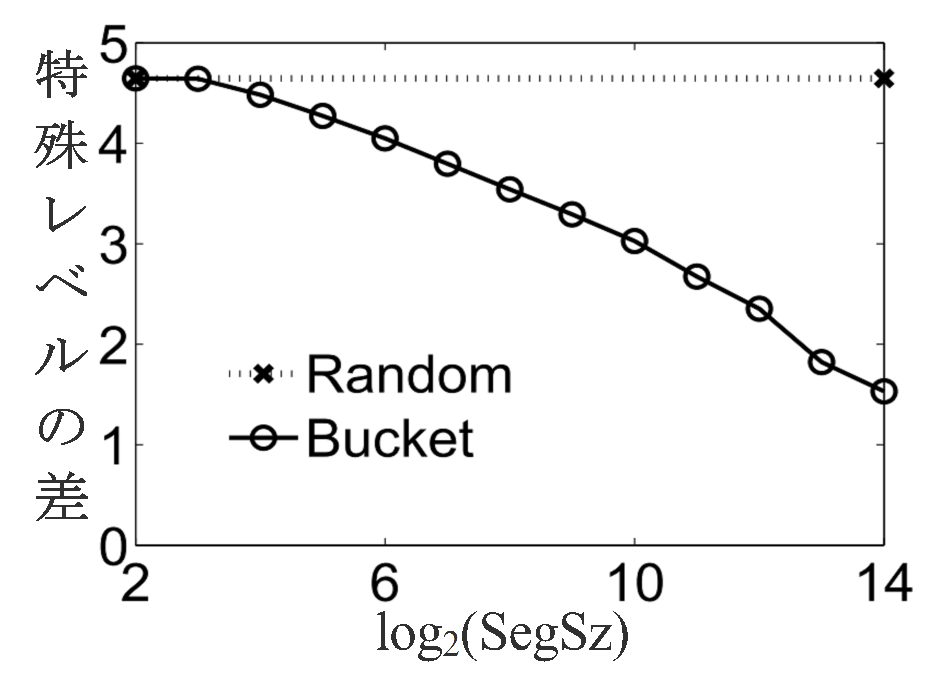
\includegraphics[width=0.9\textwidth]{rk17.eps}
\caption{特殊レベルの最大差,BktSz$=4$}
\label{fig:r1}
\end{minipage}%
\begin{minipage}[t]{0.5\linewidth}
\centering
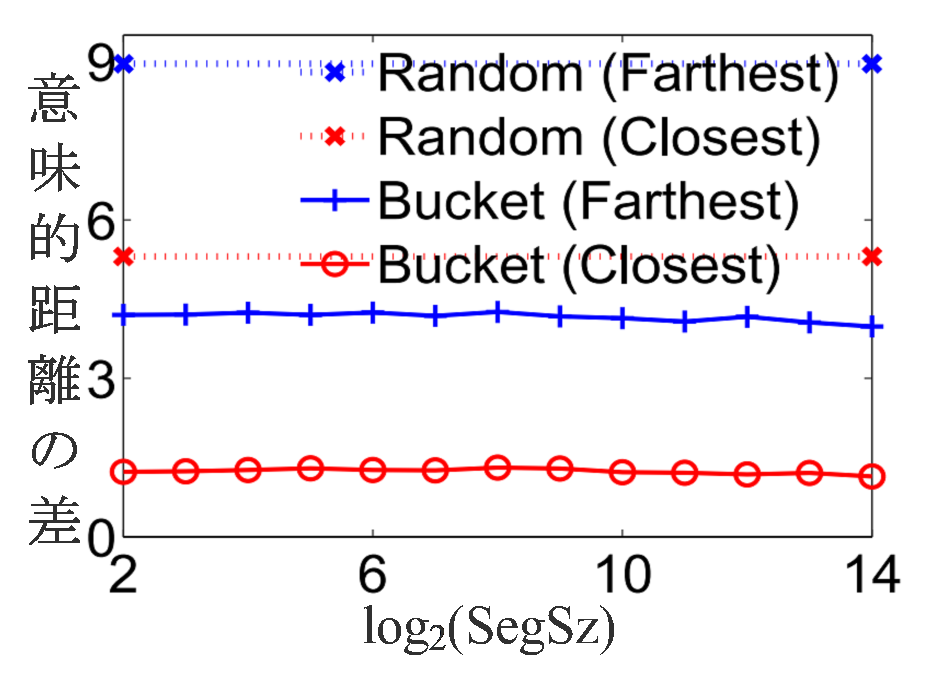
\includegraphics[width=0.9\textwidth]{rk18.eps}
\caption{単語バケツ間単語の意味的距離の差,BktSz$=4$}
\label{fig:r2}
\end{minipage}
\end{figure}

SegSzの増加によりバケツ中の単語の特殊レベルが近くなるが,意味的距離の差に影響が少ないため以下の実験はSegSzを最大値$N/$BktSzに固定する.
図\ref{fig:r3},\ref{fig:r4}がBktSzの影響を確かめる.

\begin{figure}
\begin{minipage}[t]{0.5\linewidth}
\centering
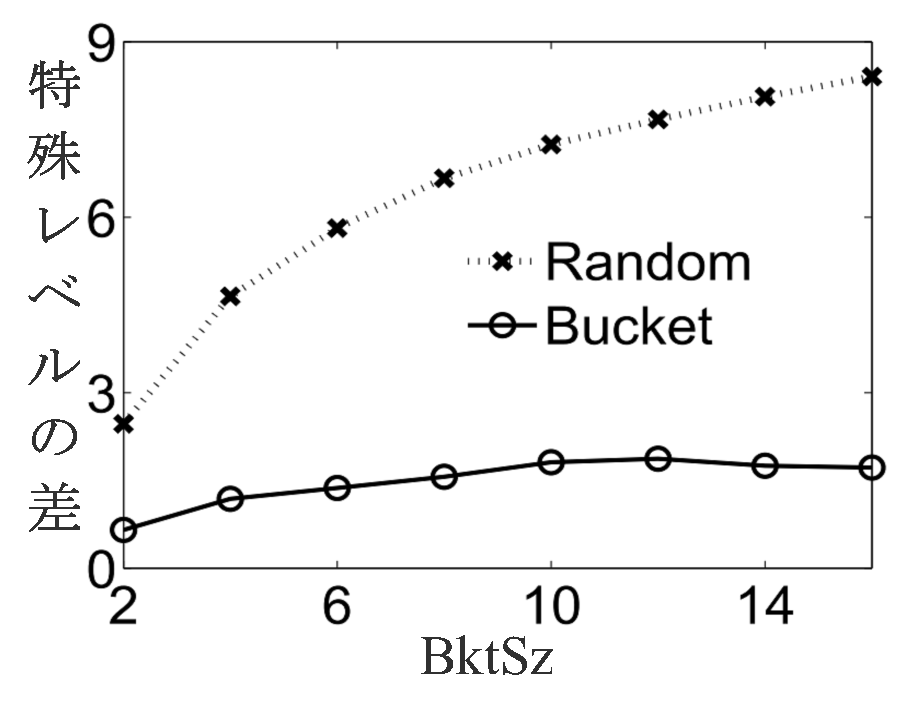
\includegraphics[width=0.9\textwidth]{rk19.eps}
\caption{特殊レベルの最大差SegSz$=N/$BktSz}
\label{fig:r3}
\end{minipage}%
\begin{minipage}[t]{0.5\linewidth}
\centering
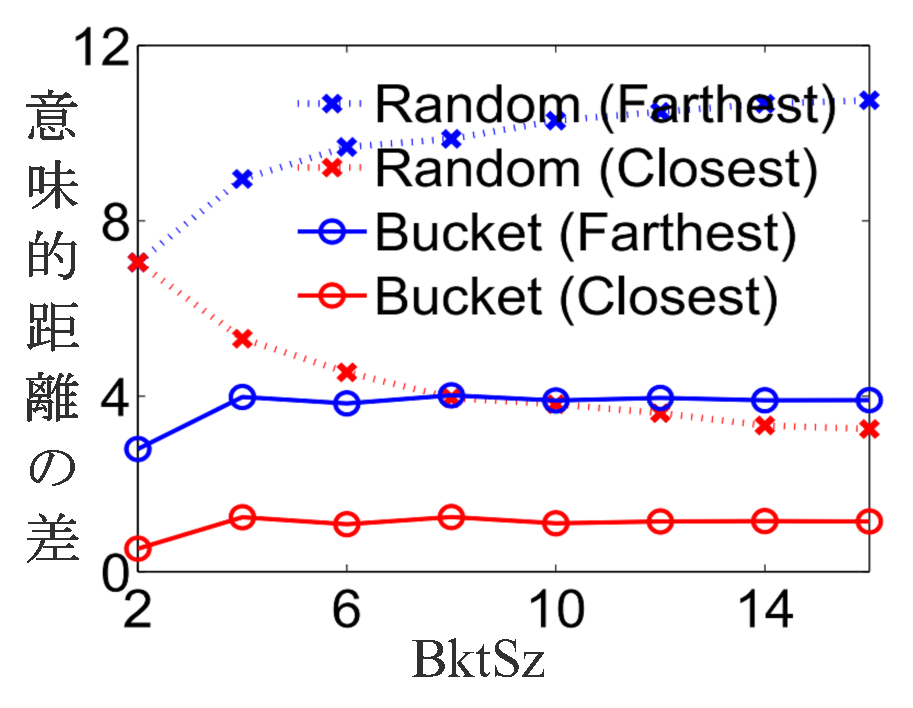
\includegraphics[width=0.9\textwidth]{rk20.eps}
\caption{単語バケツ間単語の意味的距離の差SegSz$=N/$BktSz}
\label{fig:r4}
\end{minipage}
\end{figure}


\section{メイントピック攻撃}
紹介文献では任意2つのバケツの単語間の意味的な距離の差を小くし真の質問単語間の関連性から真の質問を見破ることを防ぐ.
真の質問が一つのトピックに集中したときダミー単語も同じ特徴を表せるかどうかをNTCIR-6の特許データベース\cite{fujii_overview_2007}を用いて検証した.
特許データベースが持つ特許文章が$3,496,253$個あり,重複を除いた単語数は$2,973,096$である.特許文章が表\ref{tab:class}で表したように人手により分類されている.

\begin{table}[!hbp]
\center
\begin{tabular}{|c|c|}
\hline
&A61C 5/08A \\
\hline
セクション:A & 健康および娯楽 \\
サブセクション : 61 & 医学または獣医学:衛生学 \\
クラス: C & 歯科:口腔または歯科衛生 \\
メイングループ:5 & 歯の充填または被覆 \\
サブグループ:08 & 歯冠:その製造;口中での歯冠固定 \\
\hline
\end{tabular}
\caption{国際特許分類}\label{tab:class}
\end{table}

単語とトピックの関連性を計算するために\ref{LSI}節で紹介した潜在的意味インデキシングを用いた.
ただし,全ての特許文章と単語の行列を作り,潜在的意味インデキシングを行うには$2Tb$以上のメモリが必要であり,実践的には実行できない.
本発表では同じ分類に属する文章を一つ長い文章と見なし,単語$\cdot$分類行列に潜在的意味インデキシングを行い,単語とトピック関連性を単語のトピックベクトルで表す.
質問の全ての単語のトピックベクトルの和を質問のトピックベクトルとする.
質問,単語のトピックベクトル中一番値が高いトピックを質問,単語のメイントピックと呼ぶ.

\begin{algorithm}
\caption{メイントピック攻撃}
\begin{algorithmic}[1]
	\Require 質問:$Q=\{t_i\},$単語のトピックベクトル集合$L=\{\ell_i\}$
	\State $R=\phi, \, \ell=0$
	\State $\ell=\sum_{t_i \in Q}\ell_{t_i}$
	\State $maintopic=argmax_j \ell[j]$
	\ForAll {$bk_k \in Q $}
	\State $R=R \cup max_{t_i}q_{t_i}[maintopic]$
	\EndFor \\ 
	\Return $R$
\end{algorithmic}
\end{algorithm}

ダミー単語が真の質問単語と同様にいつのトピックに集中することが失敗したら,真の質問のメイントピックと関係が強い単語が他のトピックと関係が強い単語の数より多い,加工した質問のトピックと真の質問のトピックが一致することが考えられる.
また,一つのバケツの中の単語が意味的に遠いため,ダミー単語が真の質問単語のメイントピックとの関連性が弱いと考えられる.
メイントピック攻撃では各単語バケツ中質問のメイントピックと一番関連性が強い単語を真の質問の単語と推定する.
アルゴリズム6はその流れを表している.

本発表では特許データベース上で\cite{fujii_overview_2007}の特許検索タスクに用いた質問$2,908$個を入力としてメイントピック攻撃を実行した.
質問の平均単語数が$21.0$である.
単語の関係性に攻撃するため,SegSzが一番攻撃しづらいと考えた$1$に設定する.
全ての$60,928$個単語バケツを攻撃した結果が図\ref{fig:mt1}で表している.
単語ごとに$9$個のダミー単語を加えても$80\%$以上の確率で真の質問を見破られる.
図\ref{fig:mt2}が加工した質問のメイントピックと真の質問のメイントピックが一致する確率を表している.
質問加工により質問のメイントピックが隠すことが困難であると考えられる.

\begin{figure}
\begin{minipage}[t]{0.5\linewidth}
\centering
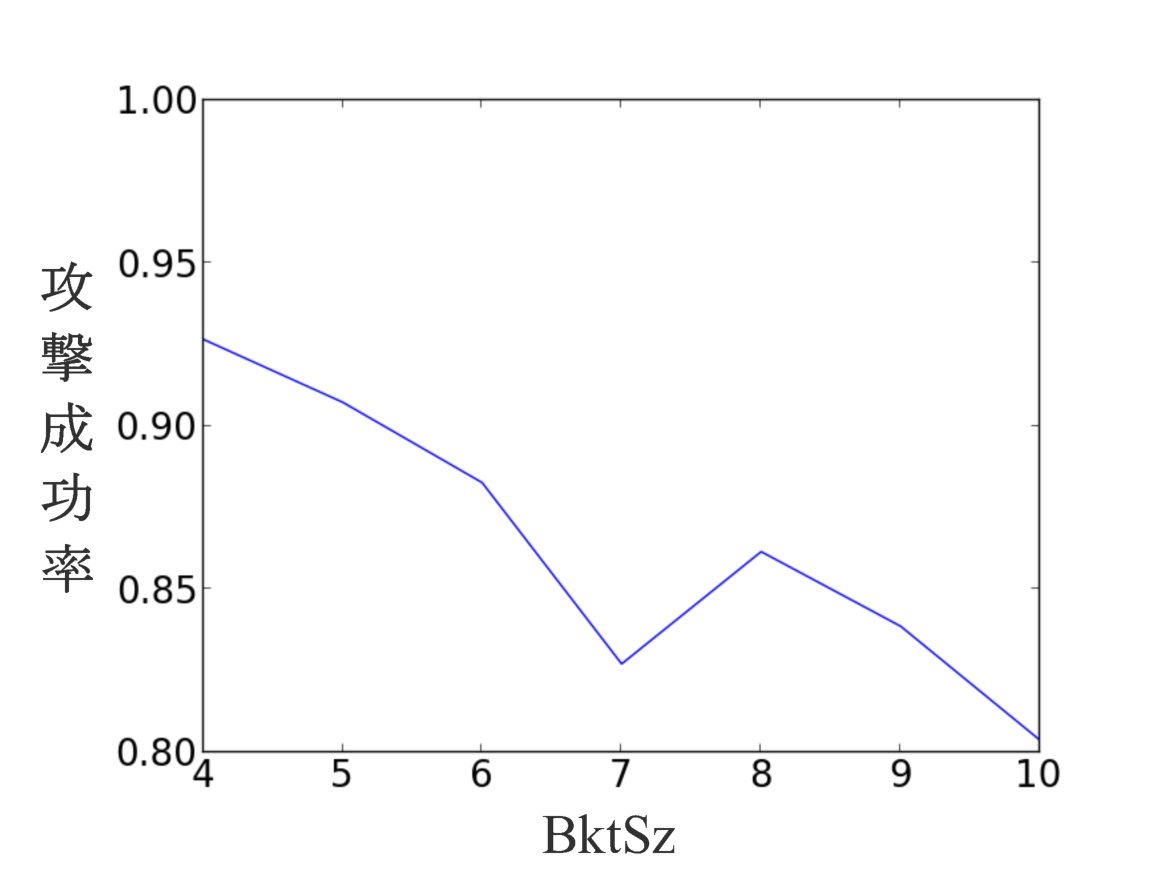
\includegraphics[width=0.9\textwidth]{rk21.eps}
\caption{単語バケツに対してメイントピック攻撃の成功率}
\label{fig:mt1}
\end{minipage}%
\begin{minipage}[t]{0.5\linewidth}
\centering
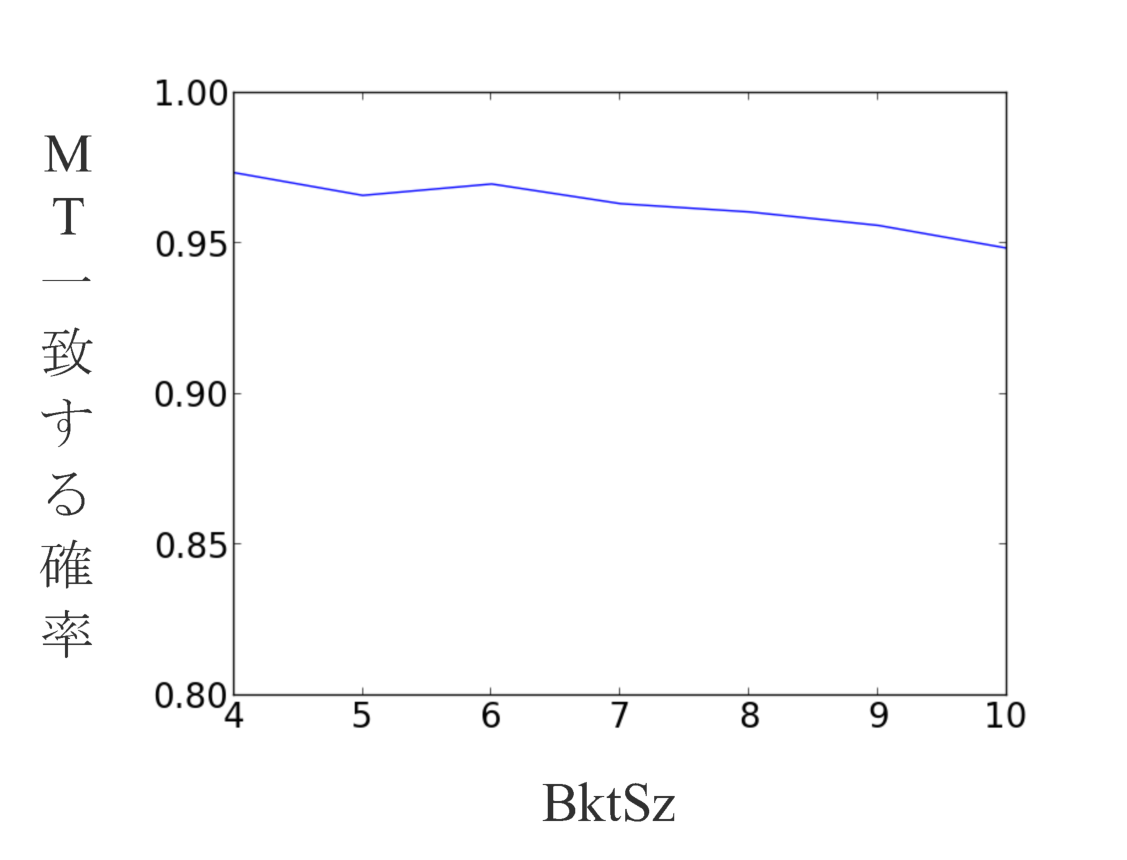
\includegraphics[width=0.9\textwidth]{rk22.eps}
\caption{加工した質問のメイントピックと真の質問のメイントピックが一致する確率}
\label{fig:mt2}
\end{minipage}
\end{figure}

\section{まとめ}
本発表では特許データベース検索に対応できるテキスト検索の質問のプライバシー保護の代表的な手法を紹介した.その手法を特許データベースで実現し,LSIを用いた攻撃手法を提案して紹介手法を評価した.質問全体ではなく単語ごとにダミー単語を加える手法は特許デーだベース検索に対応できるが,実験結果により質問加工による質問のメイントピックを保護することが困難であると考えられる.

今後の課題としては質問のメイントピックではなくサブトピックを保護する手法の提案,WordNet以外のデミー単語バケツを作るツールの提案等が挙げられる.
\bibliographystyle{tieice}
\bibliography{zotero}

\end{document}

曖昧化検索(Obfuscation Search)